


\tikzset{every picture/.style={line width=0.75pt}} %set default line width to 0.75pt        

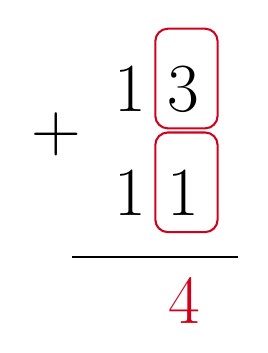
\begin{tikzpicture}[x=0.75pt,y=0.75pt,yscale=-1,xscale=1]
%uncomment if require: \path (0,300); %set diagram left start at 0, and has height of 300

%Straight Lines [id:da639216133210732] 
\draw    (230,148) -- (310,148) ;
%Rounded Rect [id:dp6218750573163438] 
\draw  [color={rgb, 255:red, 208; green, 2; blue, 27 }  ,draw opacity=1 ] (270,44) .. controls (270,40.69) and (272.69,38) .. (276,38) -- (294,38) .. controls (297.31,38) and (300,40.69) .. (300,44) -- (300,80) .. controls (300,83.31) and (297.31,86) .. (294,86) -- (276,86) .. controls (272.69,86) and (270,83.31) .. (270,80) -- cycle ;
%Rounded Rect [id:dp0945426396273431] 
\draw  [color={rgb, 255:red, 208; green, 2; blue, 27 }  ,draw opacity=1 ] (270,94) .. controls (270,90.69) and (272.69,88) .. (276,88) -- (294,88) .. controls (297.31,88) and (300,90.69) .. (300,94) -- (300,130) .. controls (300,133.31) and (297.31,136) .. (294,136) -- (276,136) .. controls (272.69,136) and (270,133.31) .. (270,130) -- cycle ;

% Text Node
\draw (249,55) node [anchor=north west][inner sep=0.75pt]  [font=\Huge] [align=left] {1 3};
% Text Node
\draw (249,105) node [anchor=north west][inner sep=0.75pt]  [font=\Huge] [align=left] {1 1};
% Text Node
\draw (209,77) node [anchor=north west][inner sep=0.75pt]  [font=\Huge] [align=left] {+};
% Text Node
\draw (275,157) node [anchor=north west][inner sep=0.75pt]  [font=\Huge,color={rgb, 255:red, 208; green, 2; blue, 27 }  ,opacity=1 ] [align=left] {4};


\end{tikzpicture}



